\chapter{FET in Horizon 2020}
This chapter focuses on the FET funding programme. Section \ref{The_Horizon_2020_programme} illustrates the Horizon 2020 initiative. Section \ref{The_FET_programme} is a description of FET in the framework of Horizon 2020. Sections \ref{FET_and_high-performing_computing} and \ref{FET_and_quantum_technologies} summarise the FET effort towards the development of quantum technologies and high-performing computers, i.e., the two most important research lines for the scope of this thesis.

\section{The Horizon 2020 programme} \label{The_Horizon_2020_programme}
Horizon 2020 is the biggest Research and Innovation programme funded by the European Union to date. It targets a smart and sustainable societal and economic growth via the development and application of scientific research. The available budget totals nearly \euro 80 billion over a seven-year period (from 2014 to 2020) \cite{Horizon2020}.

Horizon 2020 is Europe's eighth Research and Innovation programme in chronological order \cite{FP4,FP5,FP6,FP7}. The first was launched in 1984. Duration and allocated budget of each Research and Innovation programme is shown in figure \ref{FP_funds}.

\begin{figure}[!t] 
 \begin{center}
 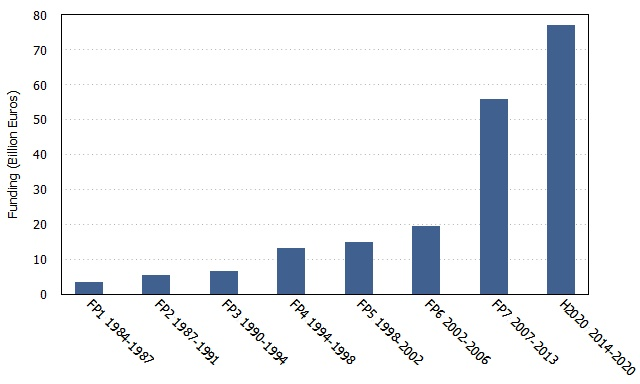
\includegraphics[scale=0.4]{Images/FP_funds.jpg}
 \caption{Duration and allocated budget of Europe's Research and Innovation programmes (also known as Framework Programmes, FP). Budgets are expressed in billion Euros. Data from \cite{FPBudget}.}
 \label{FP_funds}
 \end{center}
\end{figure}

Any natural or legal persons (e.g. universities, research organisation and companies) can apply for Horizon 2020 funding. The main categories into which applications must fit into one of the following categories: 

\begin{itemize}
 \item \textbf{Excellent Science:} this initiative supports the excellence of European scientific research on a global level and in a variety of fields \cite{ExcellentScience}.
 \item \textbf{Industrial Leadership:} this class of projects targets the development of technological innovations for the future market and the growth of European small and medium enterprises \cite{IndustrialLeadership}.
 \item \textbf{Societal Challenges:} this category focuses on priorities of the European society such as health, education, energy supply and food by combining knowledge and methods from disparate scientific fields\cite{SocietalChallenges}.  
 \item \textbf{European Institute for Innovation and Technology:} this institute is an independent European body supporting growth via the promotion of synergies in the fields of education, research and business \cite{EIT}. 
 \item \textbf{Euratom:} this pillar funds nuclear research in the framework of the decarbonisation of the energy supply \cite{Euratom}.
\end{itemize}
The Horizon 2020's budget breakdown into the aforementioned lines of action is shown in figure \ref{H2020_budget_breakdown}.

\begin{figure}[!t] 
 \begin{center}
 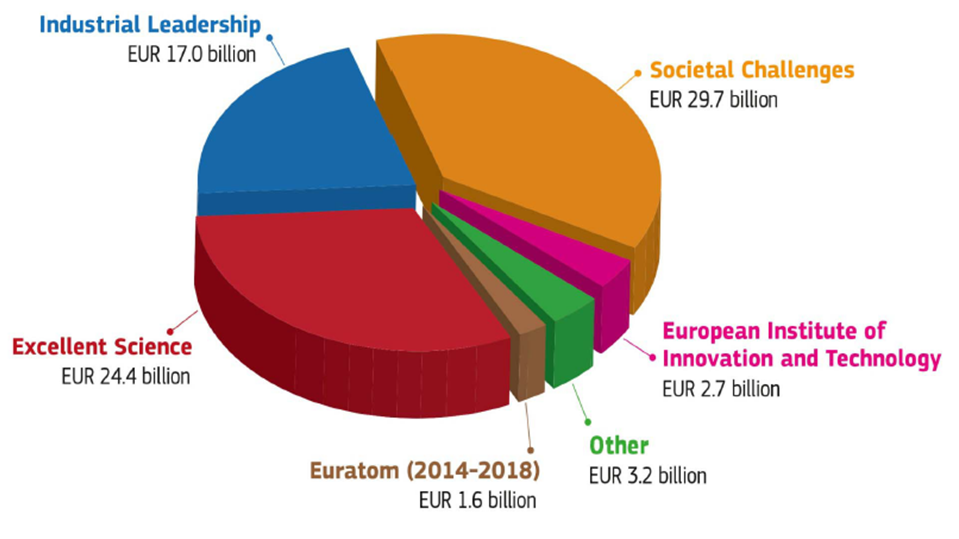
\includegraphics[scale=0.3]{Images/H2020_budget_breakdown.png}
 \caption{Budget breakdown of the Horizon 2020 programme. Original image in \cite{H2020Budget}.}
 \label{H2020_budget_breakdown}
 \end{center}
\end{figure}

\section{The FET programme} \label{The_FET_programme}
As mentioned in section \ref{The_Horizon_2020_programme}, one of the actions of Horizon 2020 is the Excellent Science programme. This initiative supports researchers and institutions developing new science and cutting-edge technology. The goal is to keep European research at the forefront of scientific innovation and discover applications to improve the citizens' life and ensure economical growth.  

\begin{table}[t]
 \begin{center}
  \begin{tabular}{cc}
   \hline 
   \hline
   Line of action & Estimated final budget \\ 
   \hline
   \hline
   ERC & 13.1 \\
   FET & 2.7 \\
   MSCA & 6.2 \\
   RI & 2.5 \\
   \hline
   \hline
  \end{tabular}
 \end{center} 
 \caption{Estimated final budget breakdown of the Excellent Science initiative. ERC stands for European Research Council; FET for Future and Emerging Technologies; MSCA for Marie Sk\l{}odowska-Curie Actions; RI for Research infrastructure. Budgets are in billion Euros. Data from \cite{OECD}.}
\label{FET_budget_breakdown} 
\end{table}

Excellent Science is based on the following pillars: 

\begin{itemize}
 \item \textbf{European Research Council:} it distributes funding in every research field to single scientists and with the requirement of scientific excellence \cite{ERC}.  
 \item \textbf{Future and Emerging Technologies (FET):} it finances collaborative research exploring visionary and radically new investigation lines \cite{FET}. 
 \item \textbf{Marie Sk\l{}odowska-Curie Actions:} this initiative assigns grants to researchers at any stage of their career and encourages mobility between countries and fields of expertise \cite{MSCA}. 
 \item \textbf{Research infrastructure:} it promotes the creation of transnational networks of research infrastructures as well as the training of qualified staff. 
\end{itemize}
The estimated final budget breakdown of Excellent Science is reported in table \ref{FET_budget_breakdown}.

\begin{figure}[!t] 
 \begin{center}
 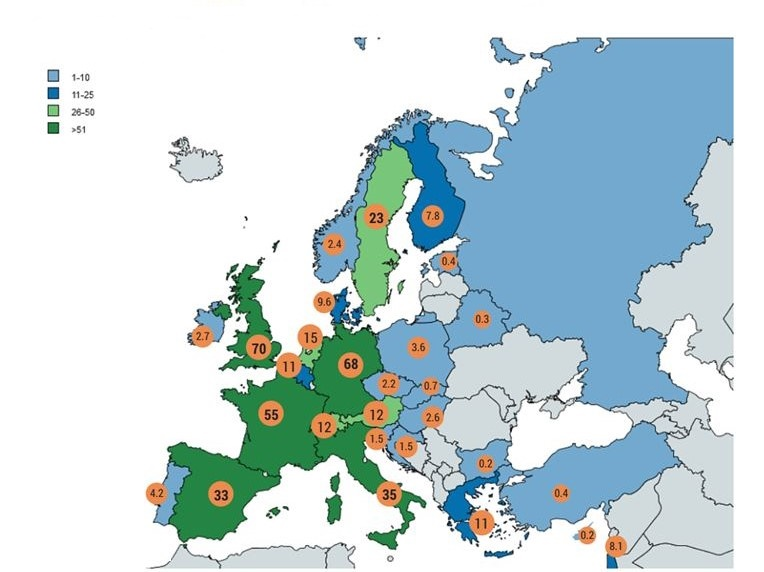
\includegraphics[scale=0.3]{Images/Country_participation_in_H2020_FET_projects.jpg}
 \caption{Participants in the Horizon 2020 FET programme on a country basis as of June 2016. Numbers correspond to FET funding in millions of euro. Colours indicate the number of participants. Adapted from image in ....}
 \label{Country_participation_in_H2020_FET_projects}
 \end{center}
\end{figure}

%image downloaded from https://ec.europa.eu/programmes/horizon2020/en/news/infographic-participation-horizon-2020-fet-projects

This thesis focuses on the communication activity of the 151 FET projects funded to date within Horizon 2020. The list of these projects is available in appendix \ref{List_of_FET_projects}. The distribution of projects participants per country as of June 2016 is shown in figure \ref{Country_participation_in_H2020_FET_projects}.

The FET funding scheme comprises three calls for applications: FET Open, FET Proactive and FET Flagship.

\subsubsection{FET Open}
The FET Open call is not bound to one specific investigation theme. However, submitted research proposals must satisfy the following ``gatekeepers": scientific and technological breakthrough; foundational; novelty; high-risk; long-term vision; interdisciplinary. 

FET Open promotes the Coordination and Support Actions (CSA) as well. These aim at identifying and fulfilling the optimal conditions for FET-related collaborative investigation. One CSA type of action is FET Innovation Launchpad, which investigates and explores possible economical and societal applications of FET results. The list of Horizon 2020 projects funded within the FET Innovation Launchpad action is reported in appendix \ref{Specific_lists_of_FET_projects}. 

\subsubsection{FET Proactive}
The FET Proactive call nurtures the birth of synergies on specific research lines by bringing together scientists from interdisciplinary fields. Considered research lines are not ready for the market yet.    

Currently, FET Proactive comprises three calls related to ``Boosting emerging technologies" and three under ``High Performance Computing". Given its relevance for this thesis, the ``High Performance Computing" FET Proactive call is illustrated in section \ref{FET_and_high-performing_computing}. 

FET Proactive invests resources also on identifying investigation roadmaps, design and distribute material for educational purposes and disseminate FET results among interested stakeholders.  

\subsubsection{FET Flagship}
FET Flagships are Europe's main research effort. They are large-scale, decade-long projects with budgets totalling one billion Euros each. The ultimate goals are to shed light on key scientific themes and apply the results to European society. To date, three FET Flagships have been approved in the Horizon 2020 programme: 

\begin{itemize}
 \item \textbf{Human Brain Project:} it targets groundbreaking steps forward in neuroscience.
 \item \textbf{Graphene:} it explores graphene's properties and possible applications.
 \item \textbf{Quantum Technologies:} it aims at developing innovative technologies based on the laws of quantum physics.
\end{itemize}
The Human Brain Project and Graphene Flagships started in April 2016. The Quantum Technologies Flagship will start running in 2018. Given its relevance for this thesis, the Quantum Technologies Flaghisp is described in section \ref{FET_and_quantum_technologies}.

\section{FET and high-performing computing} \label{FET_and_high-performing_computing}
Current and future scientific and engineering challenges require increasing levels of computational performances. The demand can be satisfied via the construction of large computer clusters and the development of suitable programming languages. The former provide higher computational power, the latter an optimal exploitation of the clusters' resources. The use of such practices is known as high-performing computing (HPC).

In terms of increasing computational power, one major HPC goal is the transition from the peta- to the exascale. This corresponds to the increase from $10^{15}$ floating point operations per second, i.e. the limit of present-day most powerful supercomputers, to $10^{18}$. The upgrade to the exascale is motivated by its major impact on all scientific fields, as it would push forward research and the development of new technology over the next decades. 

As mentioned in section \ref{The_FET_programme}, the European HPC effort is funded within the ``High Performance Computing" FET Proactive call. This call comprises three initiatives: \textit{i}) co-design of HPC systems and applications; \textit{ii}) transition to exascale computing; and \textit{iii}) exascale HPC ecosystem development. The main goals of the three initiatives are to develop the next-generation high-performing computers towards exascale and to provide access to the resources offered by supercomputers. The list of Horizon 2020 FET projects active in HPC is available in Appendix \ref{Specific_lists_of_FET_projects}.


\section{FET and quantum technologies} \label{FET_and_quantum_technologies}
Quantum technologies arise from applications of quantum physics. They are an important research topic on a global level for their potential to revolutionise human societies.

The so-called first quantum revolution started at the beginning of the past century with the development of quantum theory. The growing understanding of the atomic world led to the birth of new disciplines, such as informatics and microelectronics, and to the construction of countless fundamental tools and electronic devices. Examples range from computers and cameras to lasers and photocopy machines. The first quantum revolution played a key role in starting the knowledge era of human society.

It is believed that the second quantum revolution will be driven by the ability acquired by humankind to actively engineer the quantum world to its own purposes. This is expected to lead to a complete new class of technologies which would reshape our society. One example is the development of quantum computers. If successfully developed, such machines will be far more powerful than any present and future computer based on classical architectures. The urge for Europe to stay at the forefront of the second quantum revolution is outlined in the so-called Quantum Manifesto.

%citazione articolo arxiv https://arxiv.org/ftp/quant-ph/papers/0206/0206091.pdf

The development of quantum technologies is a central objective of the FET programme.  The list of Horizon 2020 FET projects in this field is reported in Appendix \ref{Specific_lists_of_FET_projects}. Their activity is supported by the ERANET Cofund in Quantum Technologies, a FET Proactive initiative fostering synergies and partnerships among researchers and other stakeholders. Finally, as mentioned in section \ref{The_FET_programme}, one dedicated flagship initiative will be launched in 2018. 

\section{Chapter summary} 
In this chapter, the following items have been discussed:

\begin{enumerate}
 \item Horizon 2020 is the largest research funding programme of the European Union. It is planned to run from 2014 to 2020 and has a total budget of nearly \euro 80 billion. 
 \item One funding scheme of Horizon 2020 is Future and Emerging Technologies (FET). The FET call finances visionary research projects targeting scientific breakthroughs and the development and application of radically new technologies. The estimated FET final budget will total nearly \euro 3 billion. 
 \item The development of quantum technologies is part of the FET effort. In particular, a FET Flagship on quantum technologies has been approved in 2016 by the European Commission and will start in 2018. Allocated funds sum up to \euro 1 billion. 
 \item Another major goal of the FET initiative is the development of high-performing computers. This investigation line targets a power increase in modern supercomputers of three orders of magnitude (from $10^{15}$ to $10^{18}$ floating point operations per second). The upgrade from the peta- to the exascale will provide unprecedented computational resources in practically all scientific fields.    
\end{enumerate}